\documentclass[10pt]{article}
\usepackage[
	colorlinks=true,
	linkcolor=black,
	citecolor=blue,
	urlcolor=blue
]{hyperref}
\usepackage{xcolor}
\usepackage{graphicx}
\usepackage{hyperref}



\begin{document}
\title{Iintroduction to Latex}
\maketitle
\author{Alain 13or\\
Faculty of IT\\
Adventist unversity of Central Africa\\
\texttt{tresoralain35@gmail.com}
}




\begin{abstract}
This  for just testing my abstract....
\end{abstract}

\tableofcontents

\begin{section}{Introduction}
This study we use regression analysis to estimate the fair price on financial market........\label{A}

\begin{subsection}{Backgroud}
The background of this study ...
\end{subsection}

\begin{subsection}{Objectives}
Our objectives are ...
\begin{subsubsection}{General Objective}
My General objective is ......
\end{subsubsection}

\begin{subsubsection}{Specific Objective}
My Specific objective is ......
\end{subsubsection}

\end{subsection}

\end{section}

\newpage
\begin{section}{Methodology}
this is my methodology, \href{https://www.khanacademy.org/math/statistics-probability}{See More}

\begin{itemize}
\item Monday
\item Tuesday
\end{itemize}
Alternative
\begin{enumerate}
\item Monday
\item Tuesday
\end{enumerate}
Description
\begin{description}
\item{A.} Monday
\item {B.} Tuesday

\end{description}

 \ref{A}{Back on Top}
\end{section}

\newpage
\begin{section}{Table}

\begin{table}[h!]
\centering
\caption{Student Performance}


\begin{tabular}{|c|c|c|}
\hline
Student & Marks & Grade\\
\hline
Alice & 85 &A\\
\hline
Eric & 90 &A\\
\hline
Mucyo & 50 &F\\
\hline
\end{tabular}
\end{table}

\end{section}

\begin{section}{Graphics}
\begin{figure}[h!]
\centering
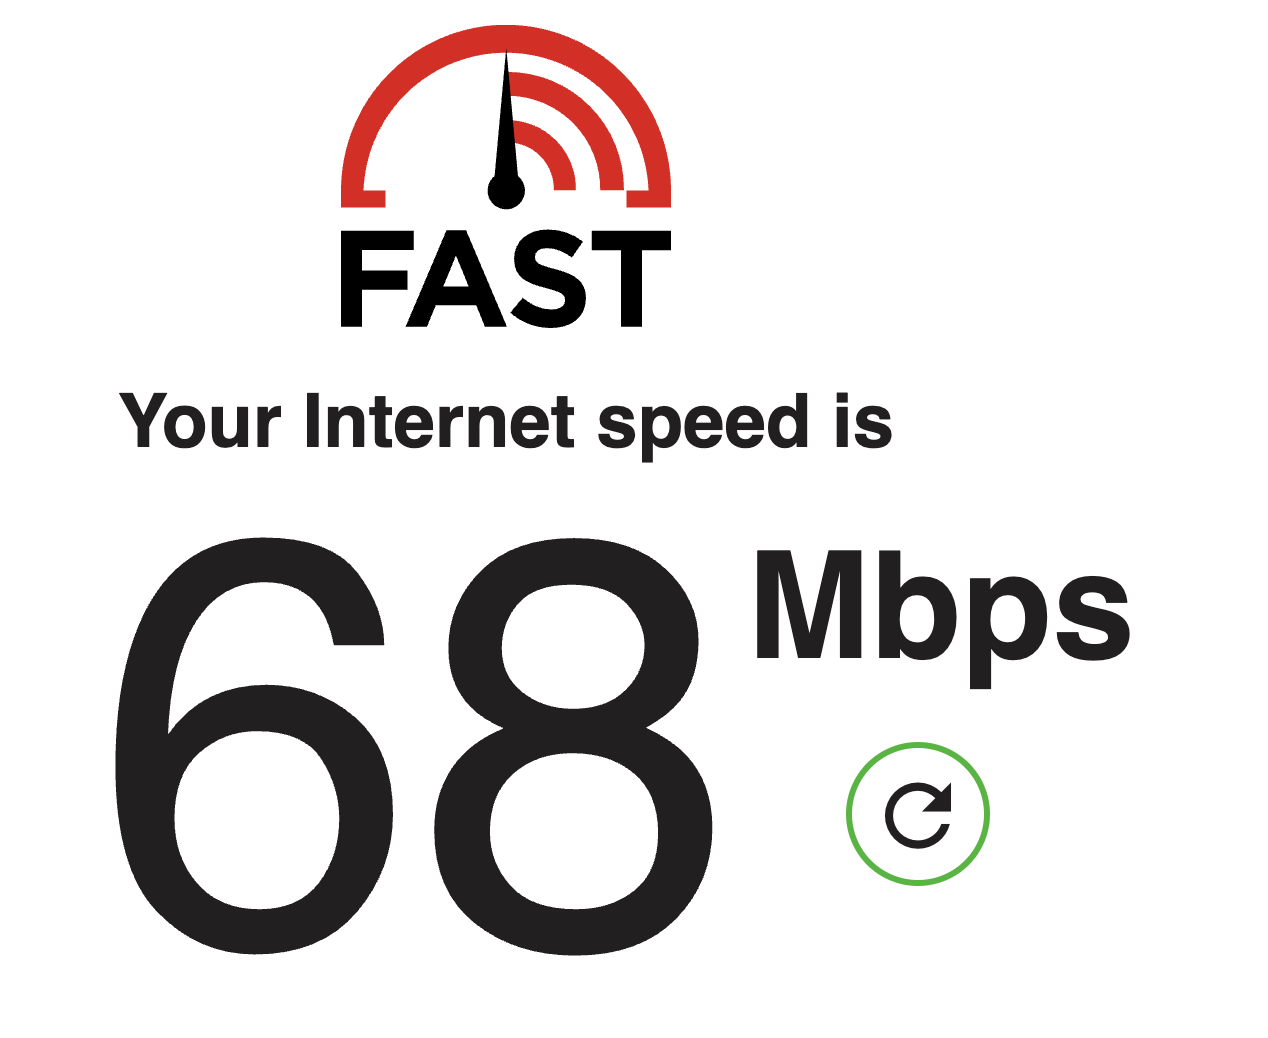
\includegraphics[width=0.6\textwidth]{logo.png}
\caption{logo}
\end{figure}

\end{section}

\end{document}